\documentclass[a4paper,10pt]{book}
\usepackage{xypic}
\usepackage[centertags]{amsmath}
\usepackage{amscd}
\usepackage{amsthm}
\usepackage{amssymb}
\usepackage{enumerate}
\usepackage{multicol}
\usepackage[english,catalan,spanish]{babel}
\usepackage[all]{xy}
\usepackage{color}
\usepackage{tikz}
\usepackage{indentfirst}
\usepackage[utf8]{inputenc}
\usepackage[T1]{fontenc}
\linespread{1.1}
\setlength{\parskip}{10pt}
\usepackage[twoside,bindingoffset=1cm]{geometry}
\usepackage{lmodern}


%% Custom packages


%%%%%%%%%%%%%%%%%%%%%%%%%%%%%%%%%%%%%%%%%%%%%%%%%%%%%%%%%%%%%%%%%%%%%%%%%%%
%%%% local definitions for this paper
%%%%%%%%%%%%%%%%%%%%%%%%%%%%%%%%%%%%%%%%%%%%%%%%%%%%%%%%%%%%%%%%%%%%%%%%%%%


%%%%%%%%%%%%%%%%%%%%%% aix{\`o} pels headings %%%%%%%%%%%%%%%%%%%%%%%%
\usepackage{fancyhdr}
\pagestyle{fancy}
\renewcommand{\chaptermark}[1]{\markboth{#1}{}}
\renewcommand{\sectionmark}[1]{\markright{\thesection\ #1}}
\fancyhf{} \fancyhead[LE,RO]{\bfseries\thepage}
\fancyhead[LO]{\bfseries\rightmark} \fancyhead[RE]{\bfseries\leftmark}

\def\paginaenblanc{\newpage%
\thispagestyle{empty}%
\vspace*{2cm}%
\newpage%
\thispagestyle{empty}%
}


%%%%%%%%%%%%%%%%%%%%%%%%%%%%%%%%%%%%%%%%%%%%%%%%%%%%%%%%%%%%%%%%%%%%%%%%%
% aux commands
%%%%%%%%%%%%%%%%%%%%%%%%%%%%%%%%%%%%%%%%%%%%%%%%%%%%%%%%%%%%%%%%%%%%%%%%%
%==========================================================================
% macros to support private authors' notes
%==========================================================================
\newif\ifprivate
\privatetrue
\def\xbar{\vskip0.09in\hrule\vskip0.06in}
\def\private#1{\ifprivate \xbar {\em #1} \xbar
\else \fi}
\def\huh{\ifprivate ??? \marginpar{\Huge ???}
\else \fi}
\def\???{\ifprivate {\bf {???}} \marginpar{\begin{center}{\Huge {\bf ?}}\end{center}}
\else \fi}
%\def\???{\ifprivate {\bf {???}} \marginpar{{\Huge {\bf ?}}}
%\else \fi}
\marginparsep1mm
\def\nota#1{\ifprivate  $\clubsuit$ \marginpar{\parbox[t]{2.4cm}{\begin{center}\tiny #1\end{center}}}
\else \fi}
\def\comment#1{\ifprivate \marginpar{\parbox[t]{2.4cm}{\begin{center}\tiny #1\end{center}}}
\else \fi}
%\def\nota#1{\ifprivate  $\clubsuit$ \marginpar{\parbox[t]{1.8cm}{\tiny #1}}
%\else \fi}
\def\privateeject{\ifprivate\eject\fi}
%\def\???{{\bf {???}} \marginpar{{\Huge {\bf ?}}} }
%%%%%%%%%%%%%%%%%%%%%%%%%%%%%%%%%%%%%%%%%%%%%%%%%%%%%%%%%%%%%%%%%%%%%%%%%%

%%%%%%%%%%%%%%%%%%%%%%%%%%%%%%%%%%%%%%%%%%%%%%%%%%%%%%%%%%%%%%%%%%%%%%%%
%%%%%%%%%%%%%%%%%%%%%%%%%%%%%%%%%%%%%%%%%%%%%%%%%%%%%%%%%%%%%%%%%%%%%%%%
\begin{document}

\pagestyle{empty}

\begin{titlepage}
\begin{center}
\begin{figure}[htb]
\begin{center}

\includegraphics[width=6cm]{assets/ub_color.pdf}
\end{center}
\end{figure}

\def\worktitle{Development of an AI-Based Tool for Molecular Subtype Classification of Invasive Ductal Breast Carcinoma Using Mammography}

\textbf{\LARGE Treball final de grau} \\
\vspace*{.5cm}
\textbf{\LARGE GRAU D'ENGINYERIA INFORM\`{A}TICA } \\
\vspace*{.5cm}
\textbf{\LARGE Facultat de Matem\`atiques i Inform\`atica\\ Universitat de Barcelona} \\
\vspace*{1.0cm}
\rule{16cm}{0.1mm}\\
\begin{Huge}
\textbf{Development of an AI-Based Tool for Molecular Subtype Classification of Invasive Ductal Breast Carcinoma Using Mammography} \\
\end{Huge}
\rule{16cm}{0.1mm}\\

\vspace{1cm}

\begin{flushright}


\vspace*{2.5cm}

\hfill

\renewcommand{\arraystretch}{1.5}
\begin{tabular}{ll}
\textbf{\small Autor:} & \textbf{\small David Bland\'on T\'orrez } \\
\textbf{\small Director:} & \textbf{\small Dr. Oliver D\'iaz Montesdeoca } \\
\textbf{\small Realitzat a:} & \textbf{\small  Departament de Matem\`{a}tiques i  Inform\`{a}tica  } \\
\textbf{\small Barcelona,} & \textbf{\small \today }
\end{tabular}

\end{flushright}

\end{center}

\end{titlepage}

%%%%%%%%%%%%%%%%%%%%%%%%%%%%%%%%%%%%%%%%%%%%%%%%%%%%%%%%%%%%%%%%%%%%%%%%%
\newpage
\selectlanguage{spanish}
\noindent \textbf{\large Resumen}

// TODO

%%%%%%%%%%%%%%%%%%%%%%%%%%%%%%%%%%%%%%%%%%%%%%%%%%%%%%%%%%%%%%%%%%%%%%%%%

%%%%%%%%%%%%%%%%%%%%%%%%%%%%%%%%%%%%%%%%%%%%%%%%%%%%%%%%%%%%%%%%%%%%%%%%%
\newpage
\selectlanguage{english}
\noindent \textbf{\large Abstract}

// TODO

%%%%%%%%%%%%%%%%%%%%%%%%%%%%%%%%%%%%%%%%%%%%%%%%%%%%%%%%%%%%%%%%%%%%%%%%%

%%%%%%%%%%%%%%%%%%%%%%%%%%%%%%%%%%%%%%%%%%%%%%%%%%%%%%%%%%%%%%%%%%%%%%%%%
\newpage
\selectlanguage{catalan}
\noindent \textbf{\large Resum}

// TODO

%%%%%%%%%%%%%%%%%%%%%%%%%%%%%%%%%%%%%%%%%%%%%%%%%%%%%%%%%%%%%%%%%%%%%%%%%
\newpage
\selectlanguage{spanish}
\noindent \textbf{\large Agradecimientos}

// TODO
%%%%%%%%%%%%%%%%%%%%%%%%%%%%%%%%%%%%%%%%%%%%%%%%%%%%%%%%%%%%%%%%%%%%%%%%%
\selectlanguage{spanish}
\pagenumbering{roman} \setcounter{page}{0}
\let\cleardoublepage\clearpage
\tableofcontents
\newpage \thispagestyle{empty}
%%%%%%%%%%%%%%%%%%%%%%%%%%%%%%%%%%%%%%%%%%%%%%%%%%%%%%%%%%%%%%%%%%%%%%%%%

\pagestyle{fancy}
\markboth{Introducción}{Introducción}
\newpage \thispagestyle{empty}
%%%%%%%%%%%%%%%%%%%%%%%%%%%%%%%%%%%%%%%%%%%%%%%%%%%%%%%%%%%%%%%%%%%%%%%%%
\mainmatter
\chapter{Introducción}
\section{Contextualización del problema}

En los últimos años, el cáncer de mama se ha consolidado como una de las principales causas de mortalidad entre las mujeres y representa el tipo de cáncer con mayor incidencia en esta población. Se estima que, en promedio, una de cada veinte mujeres a nivel mundial será diagnosticada con esta enfermedad a lo largo de su vida \cite{kim_global_2025}. Proyecciones recientes sugieren que, de mantenerse la tendencia actual, para el año 2050, se registrarán aproximadamente 3.2 millones de nuevos casos y 1.1 millones de muertes asociadas a esta patología, con un impacto especialmente significativo en los paises con bajo indice de desarrollo humano (HDI) \cite{kim_global_2025}.

En este contexto, las técnicas y herramientas de diagnóstico temprano desempeñan un papel fundamental para mejorar el pronóstico y supervicencia de las pacientes \cite{wang_early_2017}. 

Sin embargo, el cancer de mama es una enfermedad heterogénea\footnote{Diversidad celular presente dentro de un tumor (heterogeneidad intratumoral) o entre diferentes tumores en un mismo individuo (heterogeneidad intertumoral).} que puede clasificarse en diversos subtipos según características clínicas y, especialmente, moleculares \cite{orrantia-borunda_subtypes_2022}. Por lo tanto, el pronóstico, la respuesta a la terápia y las opciones de tratamiento dependen en gran medida de la correcta identificación del subtipo molecular.

Actualmente, la caracterización molecular del tumor se realiza principalmente mediante biopsia, un procedimiento invasivo y costoso que, en ocasiones, debe repetirse, lo que puede retrasar el inicio del tratamiento y aumentar la carga del paciente. Por ello, existe una necesidad creciente de desarrollar métodos no invasivos, accesibles y eficientes que permitan realizar esta tarea de manera fiable.

En este sentido, la mamografía se posiciona como herramienta clave, ya que es una técnica no invasiva, de bajo coste y ampliamente utilizada en el diagnóstico temprano del cáncer de mama. 

Con el surgimiento de las técnicas basadas en inteligencia artificial y aprendizaje profundo, la detección del cáncer de mama mediante mamografías ha experimentado un notable avance, alcanzando precisiones comparables o incluso superiores a las obtenidas por radiólogos expertos \cite{pattanaik_breast_2022, meenalochini_deep_2024, zahoor_breast_2022}. Más recientemente, estas metodologías han comenzado a aplicarse en la clasificación automática de subtipos moleculares a partir de imágenes mamográficas, lo que abre nuevas posibilidades para el desarrollo de métodos no invasivos de caracterización tumoral \cite{mota_breast_2024, ben_rabah_multimodal_2025}. 

... //TODO: Desarrollar cierre

\begin{figure}
    \centering
    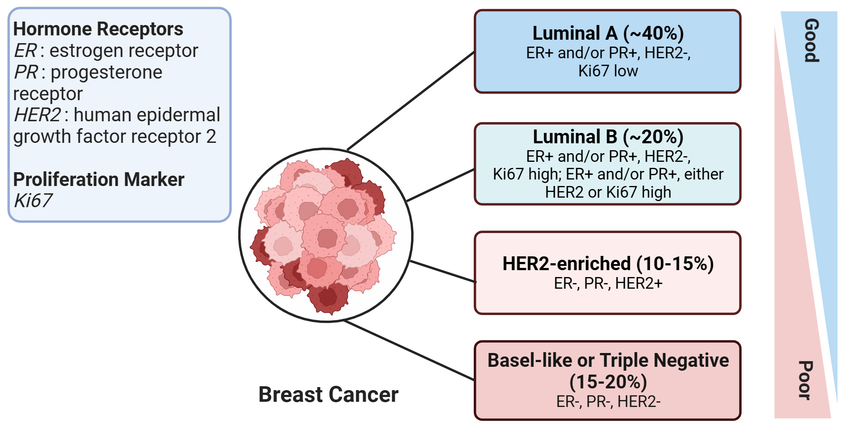
\includegraphics[width=0.8\linewidth]{reports/assets/subtypes.png}
    \caption{Los 4 subtipos moleculares del cáncer de mama y su porcentaje de relevancia \cite{harnessing_2024}}
    \label{fig:subtypes}
\end{figure}



\section{Objetivos}


El objetivo principal de este estudio es desarrollar un modelo de aprendizaje profundo capaz de clasificar subtipos moleculares de cáncer de mama utilizando exclusivamente imágenes mamográficas del \textit{Chinese Mammography Database} (CMMD), sin recurrir a metadatos clínicos o anotaciones auxiliares. Esta tarea presenta importantes desafíos, como el desbalance de clases entre los diferentes subtipos moleculares, la escasez de datos etiquetados y la ausencia de anotaciones de regiones de interés en las imágenes, factores que dificultan el aprendizaje efectivo y pueden limitar el rendimiento de los modelos de inteligencia artificial en aplicaciones médicas.

Para abordar estos retos, se evaluará de manera sistemática el rendimiento de distintas arquitecturas modernas basadas en Transformers, concretamente, Vision Transformer (ViT), Shifted-Window Transformer (SwinT) y Multi-Axis Vision Transformer (MaxViT), comparándolas con modelos convencionales basados en redes neuronales convolucionales. El enfoque en estas arquitecturas radica en que, a diferencia de las redes neuronales convolucionales tradicionales, son capaces de capturar relaciones globales y patrones complejos en las imágenes mediante mecanismos de atención, lo que resulta especialmente relevante para identificar características sutiles asociadas a la heterogeneidad molecular en las mamografías.

Se realizarán experimentos exhaustivos que incluirán estrategias como el aumento de datos adaptativo (rotaciones, espejados y transformaciones de intensidad específicas para mamografías), técnicas de \textit{oversampling} y funciones de pérdida ponderadas para abordar el desbalance de clases. El rendimiento se evaluará mediante métricas robustas como el F1-score ponderado, el área bajo la curva ROC (AUC-ROC) y la precisión balanceada, permitiendo una comparación objetiva entre arquitecturas.

Con los resultados obtenidos podremos realizar además un analisis comparativo con trabajos previos que han intentado atacar el mismo problema.

Adicionalmente, se llevará a cabo un análisis de explicabilidad del mejor modelo entrenado mediante la generación de mapas de atención y técnicas de \textit{Gradient-weighted Class Activation Mapping} (Grad-CAM). Esto permitirá identificar las regiones de las mamografías que contribuyen significativamente a las decisiones del modelo, facilitando la validación clínica y aportando \textit{insights} sobre los patrones visuales asociados a cada subtipo molecular.

... // TODO: Desarrollar cierre y estudio estadistico (p-values)

\section{Planificación}

\subsection{Tareas a desarrollar}

// TODO

\subsection{Cronograma}

//TODO



%%%%%%%%%%%%%%%%%%%%%%%%%%%%%%%%%%%%%%%%%%%%%%%%%%%%%%%%%%%%%%%%%%%%%%%%%

\chapter{Background}

\section{Breast Cancer}
\section{Molecular Subtypes}
\section{Screening Process}
\section{Mammography}


\chapter{Technology Review}


\chapter{Methodology}
\section{CMMD Dataset}
\section{Image Preprocessing}

\chapter{Results and Discussion}
\section{Results}

\chapter{Conclusions and Future Work}

%%%%%%%%%%%%%%%%%%%%%%%%%%%%%%%%%%%%%%%%%%%%%%%%%%%%%%%%%%%%%%%%%%%%%%%%%
\backmatter
\selectlanguage{spanish}
\addcontentsline{toc}{chapter}{Bibliografía}
\bibliographystyle{ieeetr}
\bibliography{references}


\end{document}
